\documentclass[journal]{vgtc} 
\usepackage{hs-vis_ws1819}
\usepackage{url}


%% Please note that the use of figures other than the optional teaser
%% is not permitted on the first page of the journal version.  Figures
%% should begin on the second page and be in CMYK or Grey scale
%% format, otherwise, colour shifting may occur during the printing
%% process.  Papers submitted with figures other than the optional
%% teaser on the first page will be refused.

%% These three lines bring in essential packages: ``mathptmx'' for
%% Type 1 typefaces, ``graphicx'' for inclusion of EPS figures. and
%% ``times'' for proper handling of the times font family.

\usepackage{mathptmx} 
\usepackage{graphicx}
\usepackage{times}
\usepackage[space]{grffile}
\usepackage{hyperref}


%% allow for this line if you want the electronic option to work
%% properly
\vgtcinsertpkg


%% author name
\author{Dominik Sellenthin \and Christian Stegmaier \and Gariharan Kanthasamy}

%% paper title
\title{OpenGL-basiertes Software Occlusion Culling zur Beschleunigung des 3D-Renderings gro{\ss}er Datenmengen und komplexer Szenen}

%% short title for header
\shorttitle{Software Occlusion Culling}


%% Abstract section.
\abstract{%

In Bereichen des 3D-Rendering, sei es in der wissenschaftlichen Visualisierung oder in Computerspielen, ist die Rechenleistung der Grafikkarte schnell an ihrer Grenze, w"ahrend die CPU kaum in Anspruch genommen wird.
Es werden daher Techniken ben"otigt, die den Aufwand beim Rendern so gering wie m"oglich halten und gleichzeitig der st"andig zunehmenden Dynamik gerecht werden.
Eine dieser Techniken ist das Software Occlusion Culling (SOC).
Ziel des Occlusion Cullings ist es, komplett parallel zum GPU-Rendering des aktuellen Frames, festzustellen, welche Objekte in der kommenden Szene zu sehen sind und welche Objekte nicht gerendert werden m"ussen.
Damit die GPU entlastet wird, ist es W"unschenswert, die Berechnungen des Occlusion Cullings auf die CPU auszulagern.
Um das zu erreichen und um die vollst"andige Rechenleistung moderner Multi-Core CPUs zu gew"ahrleisten, wird in dieser Arbeit ein bereits vorhandener Software-Rasterierer, Mesa 3D, verwendet, der zus"atzlich die OpenGL API zur Verf"ugung stellt.
In dieser Arbeit wird daher in einem von Intel entwickelten SOC-Framework eine auf Mesa-3D basierende Occlusion Culling Technik implementiert und folglich auf ihre Tauglichkeit mit bereits im Framework existierenden Techniken verglichen.
} % end of abstract


%% Uncomment below to include a (optional) teaser figure.
\teaser{ \centering
  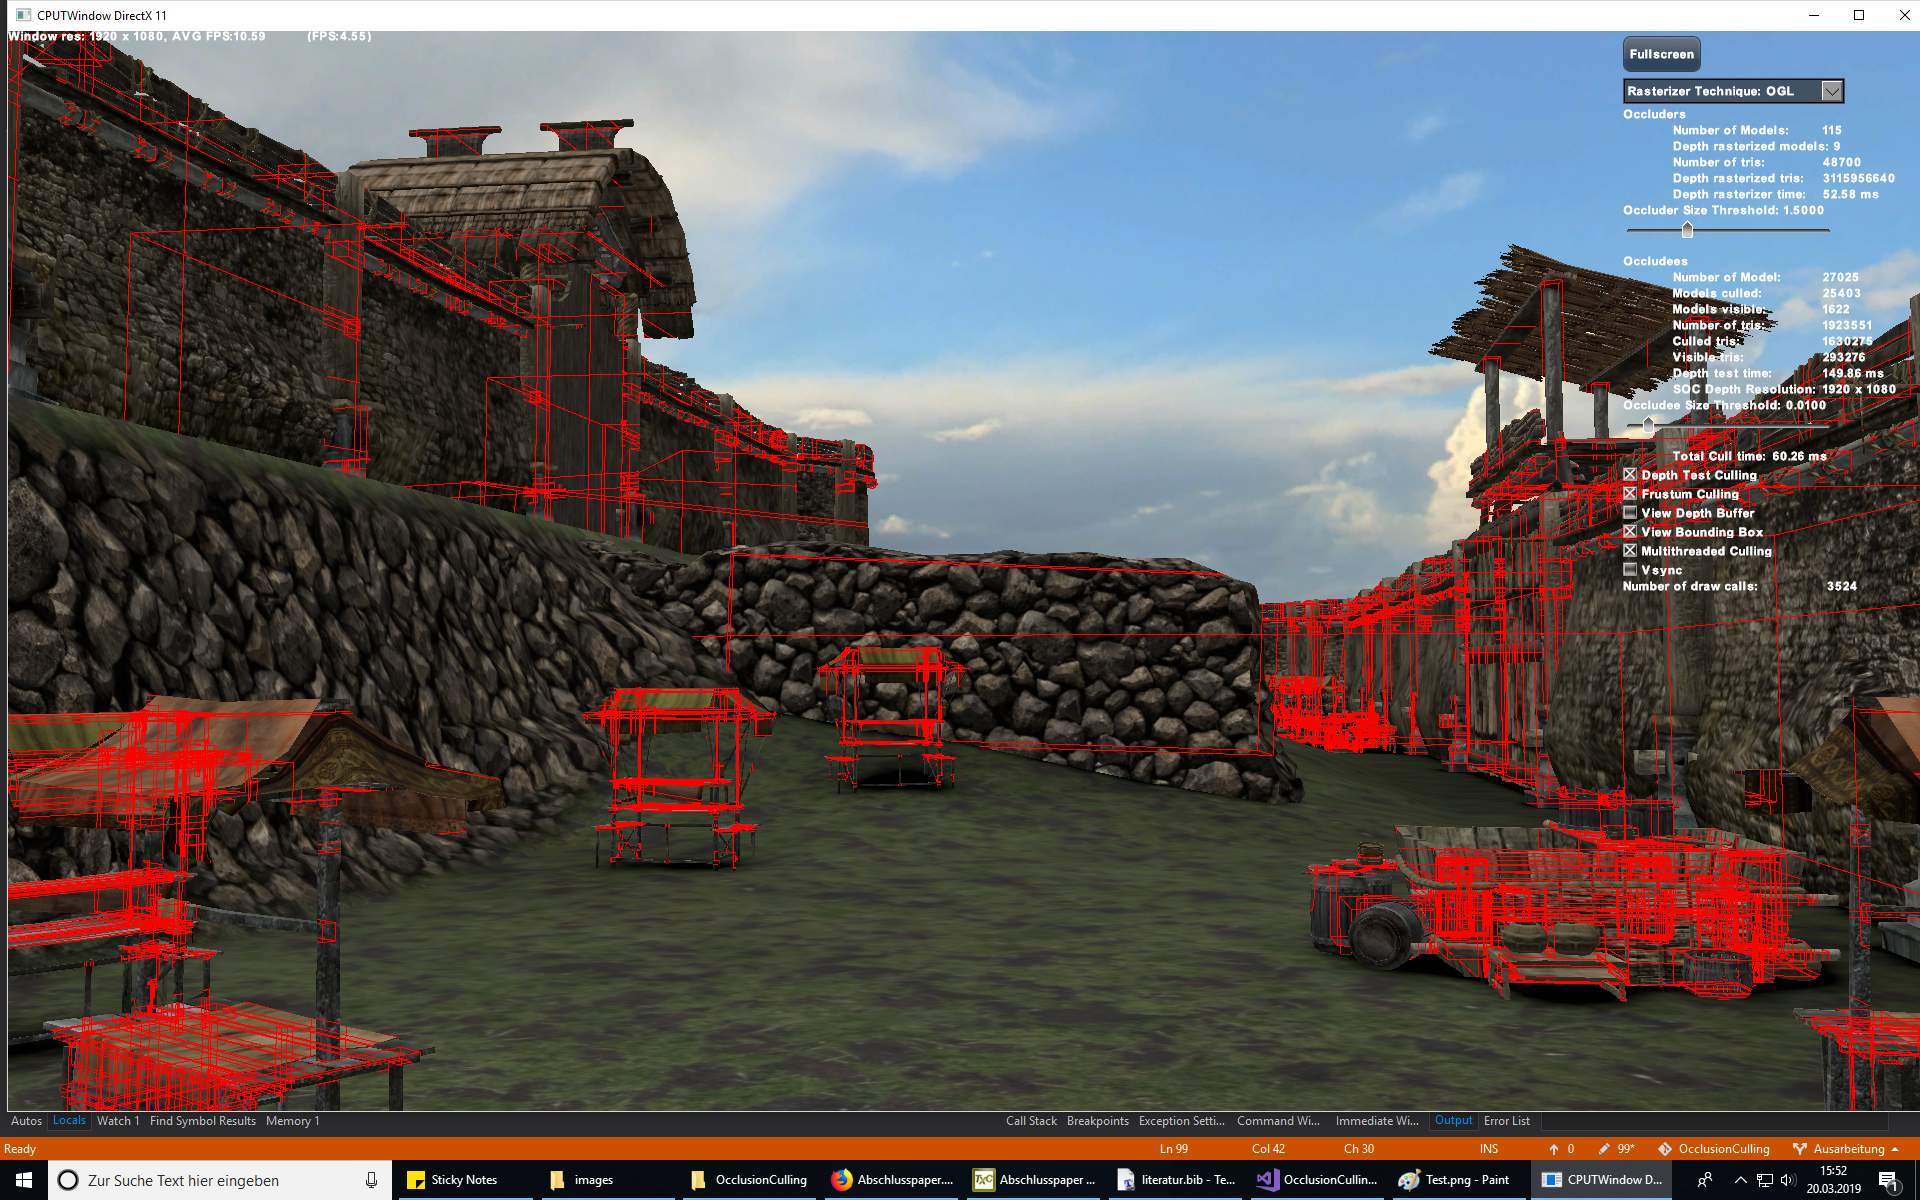
\includegraphics[width=\columnwidth]{images/Base1AABB.png}%
	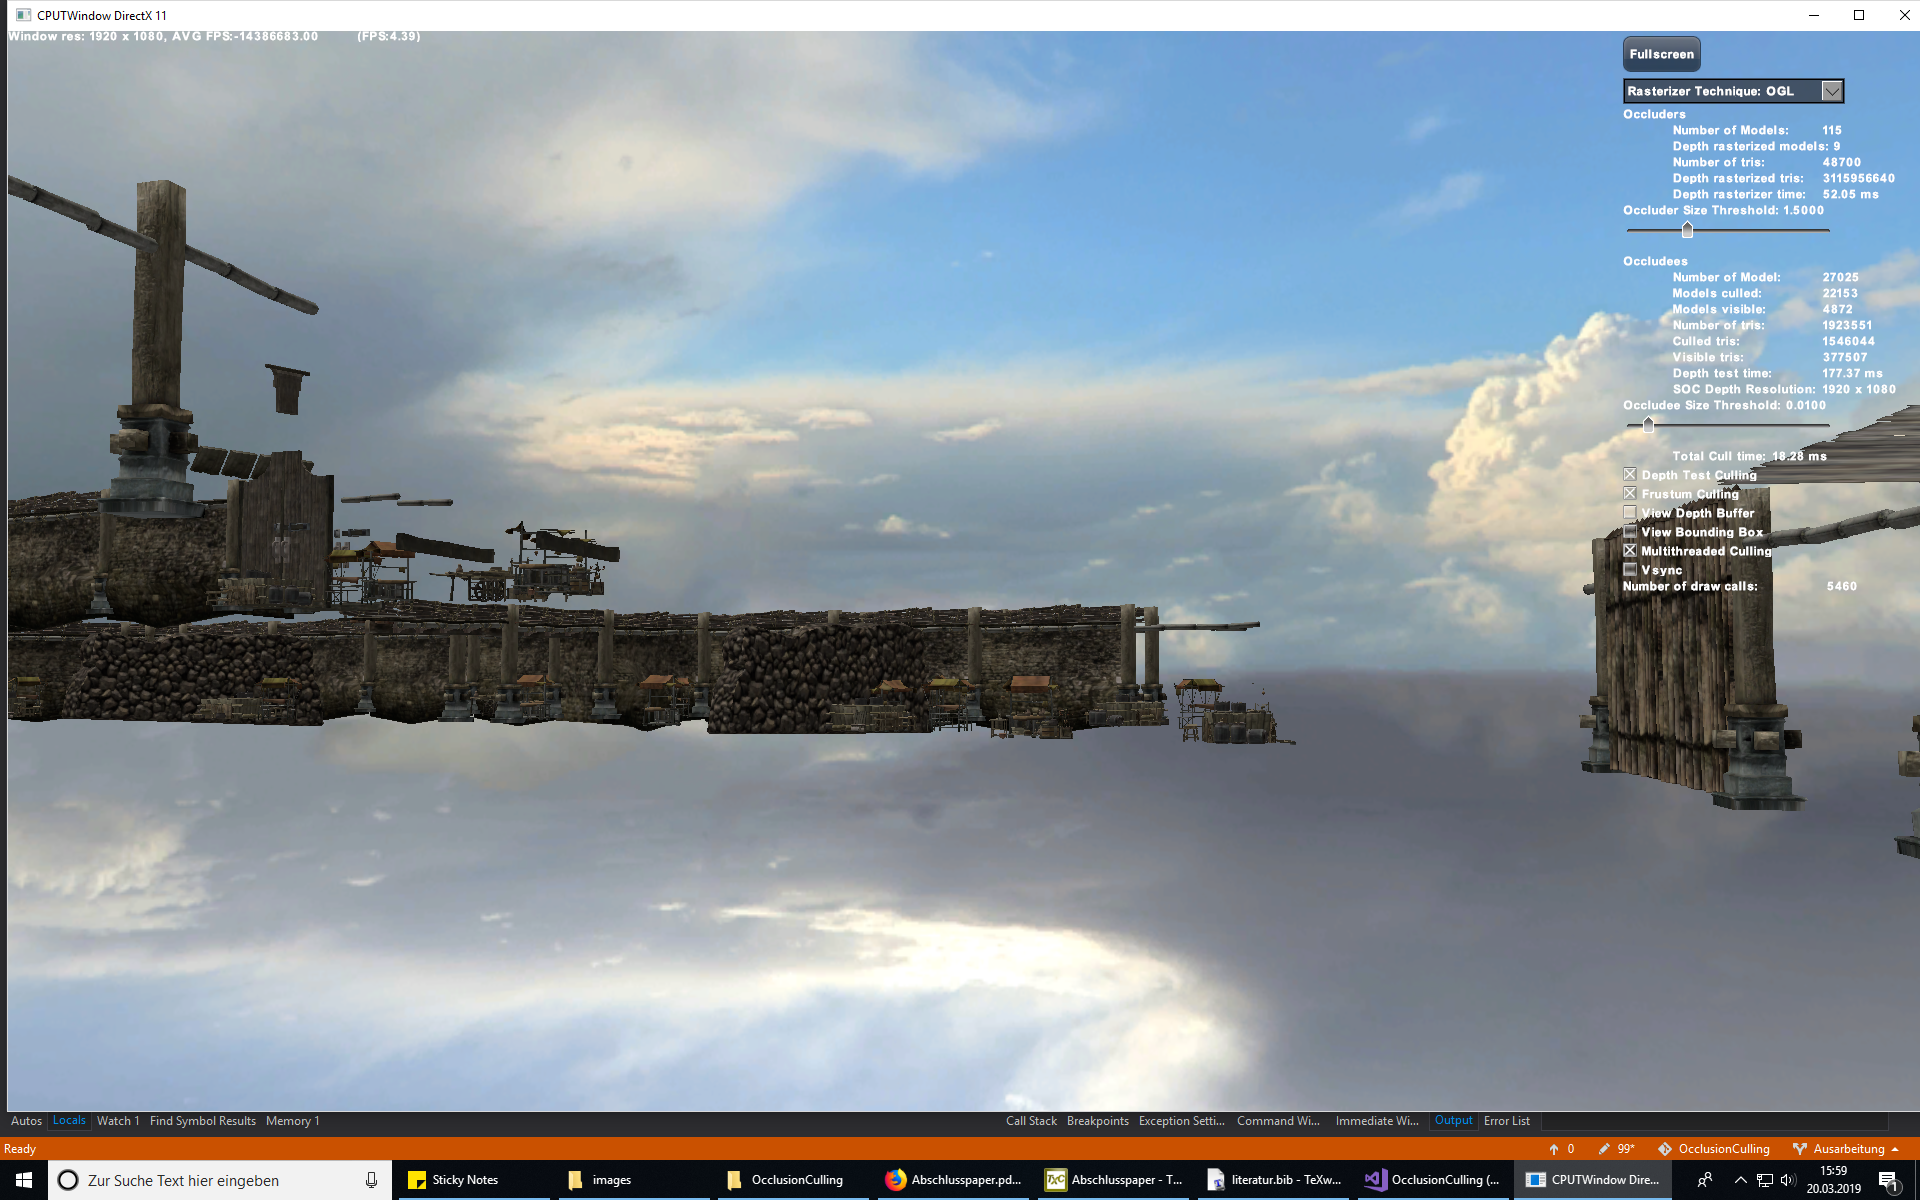
\includegraphics[width=\columnwidth]{images/Base1Invert.png}%
	\caption{Links: Testergebnisbild nach einem erfolgreichen Durchlauf der OGL-Methode aus der verwendeten Intel-Testszene. Rote Linien um Objekte stellen die Axis Aligned Bounding Box des jeweiligen Objekts dar. Rechts: Bild aller Objekte, die beim Occlusion Culling als verdeckt klassifiziert wurden und im linken Bild nicht gerendert wurden.}%
	\label{fig:teaser}
}


%%%%%%%%%%%%%%%%%%%%%%%%%%%%%%%%%%%%%%%%%%%%%%%%%%%%%%%%%%%%%%%%
%%%%%%%%%%%%%%%%%%%%%% START OF THE PAPER %%%%%%%%%%%%%%%%%%%%%%
%%%%%%%%%%%%%%%%%%%%%%%%%%%%%%%%%%%%%%%%%%%%%%%%%%%%%%%%%%%%%%%%

\begin{document}

%% The ``\maketitle'' command must be the first command after the
%% ``\begin{document}'' command. It prepares and prints the title
%%   block.

%%   the only exception to this rule is the \firstsection command
\firstsection{Einleitung}

\maketitle

Heutige Anwendungen haben immer h"ohere Anspr"uche an die Leistung der Engines(?) und der Wunsch nach besserer Performanz und h"oheren Bildraten (frames per second, FPS) ist gro{\ss}.
Hinzukommt, dass in modernen Anwendungen die zu rendernden Szenen immer weniger statisch und immer mehr dynamisch werden, wie es beispielsweise in Computerspielen der Fall ist.
Um dieser Dynamik gerecht zu werden, wird sich von Verfahren mit potenziellen Sichtbarkeitsmengen entfernt \cite{MSOC} und es wird sich einer Methode namens \textit{Occlusion Culling} (\textit{to occlude = verdecken, to cull = aussondern, herausfiltern}) bedient.
Ziel des Occlusion Cullings ist es, noch vor dem Rendering der n"achsten Szene, herauszufinden, welche Objekte in der kommenden Szene sichtbar sind und welche nicht.
Im Wesentlichen gilt es dabei zuerst mit einer ausgew"ahlten Teilmenge der Objekte einen geeigneten Tiefenpuffer (Z-Buffer) zu generieren und darauffolgend mit Hilfe von Occlusion Queries alle Objekte zu bestimmen, die noch sichtbar sind (auch Z-Buffering oder Tiefentest genannt).
Das Ergebnis der Occlusion Queries kann anschlie{\ss}end ohne nennenswerte Latenz verwendet werden, um der GPU mitzuteilen, welche Objekte gerendert werden sollen, so dass unn"otiger Rechenaufwand der GPU vermieden wird.\\

Bei Anwendungen, die ohnehin schon enormen Rechenaufwand ben"otigen und die maximale Rechenkapazit"at der Grafikkarte schnell ausreizen, ist es schwierig den zus"atzlichen Mehraufwand ebenfalls der Grafikkarte aufzuerlegen.
Es bietet sich daher an, den Mehraufwand dem wenig genutzten Prozessor zu "ubergeben, der dann komplett parallel zur Grafikkarte das Occlusion Culling in einem Vorverarbeitungsschritt durchf"uhren soll, siehe Abb.\ \ref{fig:ablauf}.

\begin{figure}%
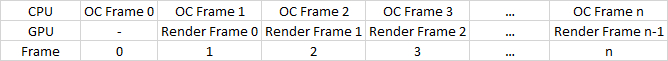
\includegraphics[width=\columnwidth]{images/Ablauf.PNG}%
\caption{W"ahrend ein Frame gerendert wird, berechnet der Prozessor parallel zum Rendering bereits, welche Objekte in der n"achsten Szene zu sehen sind.}%
\label{fig:ablauf}%
\end{figure}

Moderne Prozessoren besitzen mittlerweile einige separat nutzbare Kerne, die parallel verwendet werden k"onnen, um das Occlusion Culling so effektiv und effizient wie m"oglich zu implementieren.
Damit die gesamte Rechenleistung der Prozessoren auch genutzt wird, wird in dieser Arbeit auf den Software-Rasterisierer Mesa 3D zur"uckgegriffen, der au{\ss}erdem mit der bew"ahrten OpenGL API arbeitet. \\

Implementiert wurde die OGL-Methode in einem Software Occlusion Culling (SOC) Framework, das von Intel frei zur Verf"ugung gestellt wird \cite{SOCF}.
Das Framework eignet sich sehr gut f"ur die Implementierung einer neuen SOC-Methode, da es sowohl essentielle Ablaufstrukturen als auch eine ausreichend gro{\ss}e und komplexe Testszene zur Verf"ugung stellt, mit der eine Evaluation der OGL-Methode erm"oglicht wird, siehe Abb.\ \ref{fig:teaser} links.


\section{Related Work}
Diese Arbeit orientiert sich stark an Intels SOC-Framework, in das die in dieser Arbeit entwickelte OGL-Methode eingebettet wurde.
Da das Framework bereits alle notwendigen Strukturen f"ur schon bestehende Methoden besitzt (siehe Abb.\ \ref{fig:ablaufframework}), gestaltet sich die Erweiterung um eine weitere Methode gr"o{\ss}tenteils unkompliziert. 
\begin{figure}%
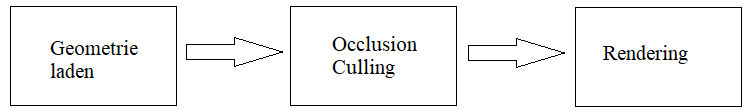
\includegraphics[width=\columnwidth]{images/AblaufFramework.png}%
\caption{Verwende gr"o{\ss}tenteils vorhandene Strukturen, um die verwendete Geometrie zu laden. Anschlie{\ss}end erfolgt das Culling durch die neue OGL-Culling-Methode. Zum Schluss wird die nicht gecullte Geometrie an das Framework zur"uckgegeben, damit das Ergebnis gerendert wird.}%
\label{fig:ablaufframework}%
\end{figure}
Hinzukommen lediglich Ver"anderungen der Routinen zum Laden der Testszene und die Implementierung des Cullings selber.
Vorhanden sind unter anderem Methoden, die mit \textit{Streaming SIMD Extension} (SSE) und \textit{Intel Advanced Vector Extension} (AVX) arbeiten.
Au{\ss}erdem ist noch eine optimierte Variante der AVX-Technik vorhanden, \textit{Masked Software Occlusion Culling} (MSOC) \cite{MSOC}, die mit einer abgewandelten Form des hierarchischen Z-Buffers (HiZ) \cite{HiZ} arbeitet, der durch einen Software-Rasterisierer berechnet wird.

Hasselgren et al. \cite{MSOC} stellen in ihrer Arbeit einen Algorithmus vor, der durch seinen effizienten HiZ die Performanz signifikant verbessert.
Anstatt wie in fr"uheren Arbeiten Pixel als kleinste Einheit zu betrachten, werden nun \textit{Kacheln} verwendet.
Kacheln sind dabei lediglich eine Zusammenfassung mehrerer aneinanderliegender Pixel.
Da AVX2 erm"oglicht, 8 SIMD Instruktionen mit 32-Bit Pr"azision auszuf"uhren, wurde f"ur die Kacheln eine Gr"o\ss{}e von 32x8 Pixeln gew"ahlt.
Indem Bitmasken von rechts und links in die Kacheln geschoben werden, wird am Ende eine Abdeckungsmaske erhalten, die angibt, welche Pixel in einer Kachel verdeckt werden \cite{MSOC}.
W"ahrend ihr Algorithmus keine 100\% Pr"azision garantiert - \textit{false positives} sind m"oglich - bewegt sich der Fehler in gleicher Gr"o\ss{}enordnung wie bei bisherigen Algorithmen.
Ein wichtiger Faktor f"ur die Performanz ihres Algorithmus ist die Reihenfolge, in der die Objekte gerendert werden.
Die Objekte sollten bestm"oglichst von vorne nach hinten gerendert werden.
Dadurch werden die wichtigsten Occluder als erstes rasterisiert (dargestellt) und f"ur den Fall, dass die Zeit f"ur Occlusion Culling begrenzt ist, wird trotzdem ein nahezu optimales Ergebnis erzielt \cite{MSOC}.\\

Bei einem Vergleich zwischen einem HiZ-Algorithmus und dem MSOC - bei voller Aufl"osung (1920x1080 Pixel) und Single-Core Performanz - geht hervor, dass der MSOC-Algorithmus 2\% weniger Dreiecke als der HiZ wegwirft, aber dennoch eine bessere Performanz erzielt \cite{MSOC}.
Mit beiden Occlusion Culling Algorithmen kann eine 1,5-7x schnellere Total Frame Time gegen"uber Rendering mit nur Frustum Culling erreicht werden.
In einem zweiten Test in einer wesentlich komplexeren Szene mit 143k Occluder-Meshes ist die Occlusion Culling Time des MSOC-Algorithmus zeitweise bis zu 10x schneller als die des HiZ-Algorithmus \cite{MSOC}.
Die Skalierbarkeit des MSOC is der des HiZ deutlich "uberlegen. Mit steigender Gr"o"se der Dreiecke steigt auch der Performanzunterschied zwischen dem MSOC und dem HiZ.
Im Allgemeinen soll der MSOC-Algorithmus 3x schneller sein und gleichzeitig 98\% aller Dreiecke wegwerfen als die bisherigen Algorithmen bei einem nur geringen Memory Overhead \cite{MSOC}.

\section{Software Occlusion Culling}
Die Menge der Objekte, die es zu Rendern gilt, wird in zwei Mengen aufgeteilt.
Zum einen gibt es die \textit{Occluder}. Occluder sind eine Menge von Objekten, die gro{\ss} genug sind, dass es wahrscheinlich ist, dass sie andere Objekte verdecken.
Zum anderen gibt es \textit{Occludees}. Occludees sind all diejenigen Objekte die potenziell von Occludern verdeckt werden (das hei{\ss}t, sie beinhalten ebenfalls alle Occluder).
\begin{figure}%
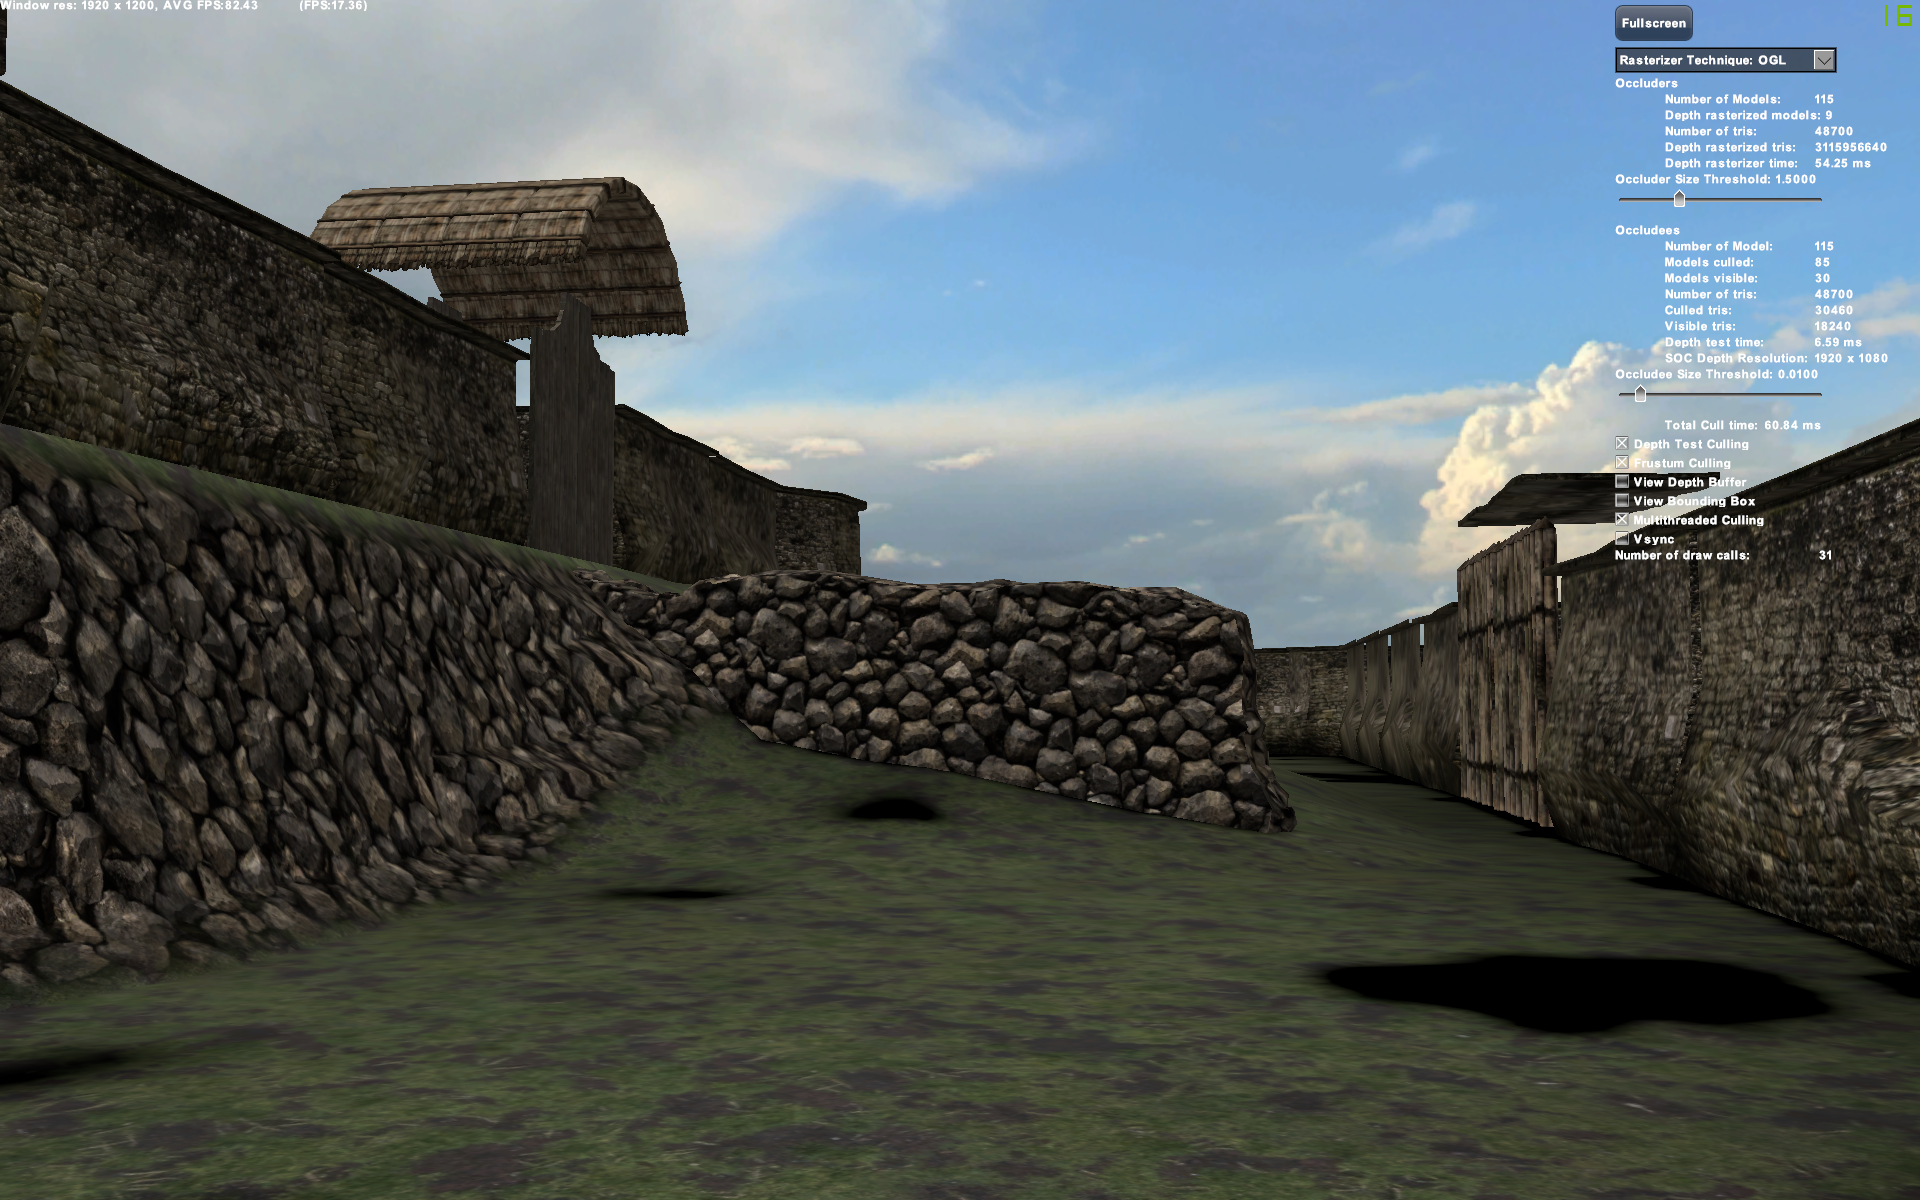
\includegraphics[width=0.5\columnwidth]{images/Occluder.png}%
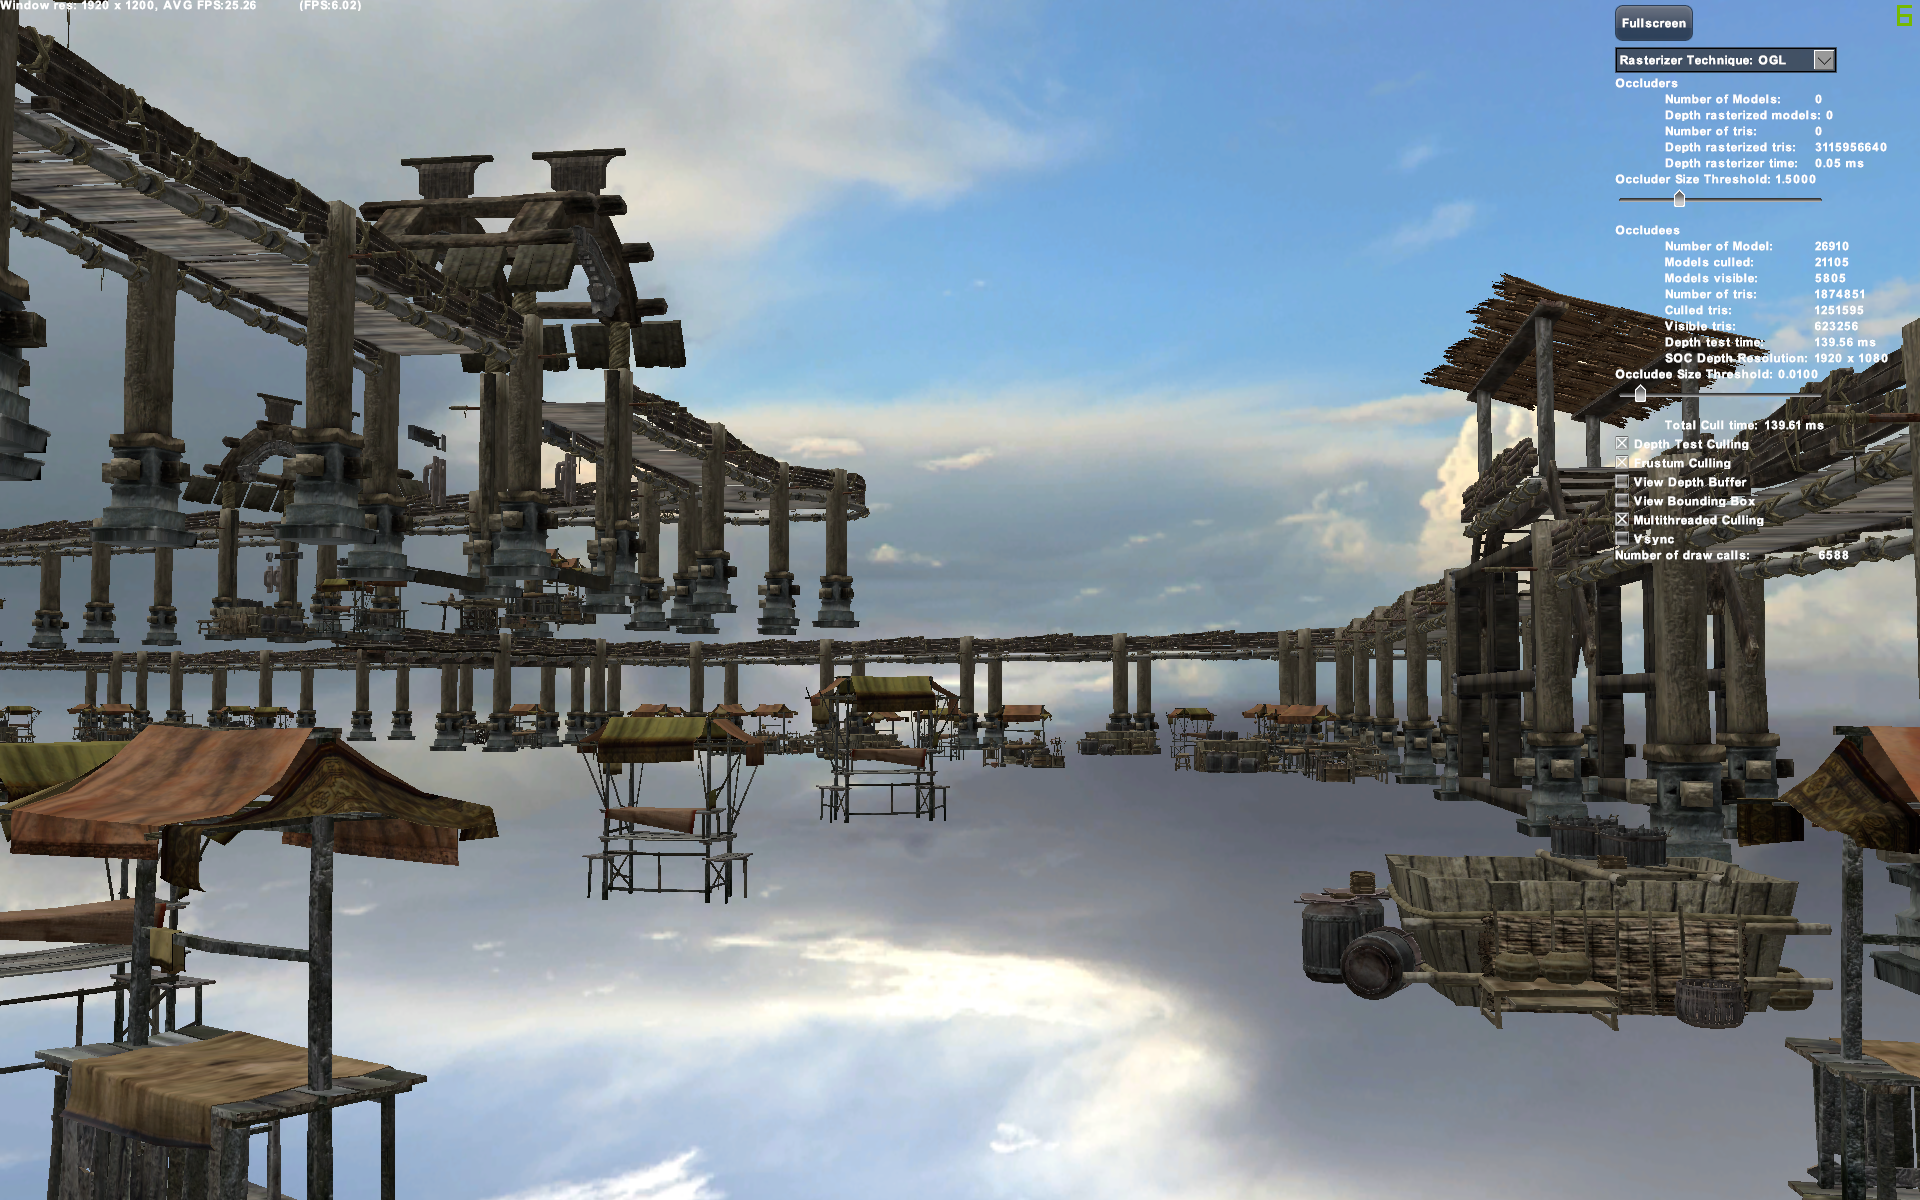
\includegraphics[width=0.5\columnwidth]{images/Occludees.png}%
\caption{Links: Menge der Occluder ohne Occludees, die in dieser Kameraeinstellung zu sehen sind, vgl. Abb.\ \ref{fig:teaser} linkes Bild. Rechts: Testszene ohne Occluder, es sind ausschlie{\ss}lich Occludees zu sehen, vgl. ebenfalls Abb.\ \ref{fig:teaser}.}%
\label{fig:objects}%
\end{figure}
Sowohl Occluder als auch Occludees liegen dabei in zwei Formen vor.
Einmal als Netz, bestehend aus Punkten (Mesh), das zur exakten Darstellung des Objekts in der gerenderten Szene dient und einmal in Form einer \textit{Axis Aligned Bounding Box} (AABB), die sowohl zum Frustum Culling als auch zum (Tiefen-)Rasterisieren verwendet wird.
AABBs eignen sich wegen ihrer einfachen geometrischen Form sehr gut, um erste grobe Tests durchzuf"uhren, ob ein Objekt "uberhaupt von der Kamera gesehen werden kann (Frustum Culling) und dementsprechend f"ur die folgende Rasterisierung beim Occlusion Culling in Frage kommt. \\

Occlusion Culling besteht im Wesentlichen aus zwei Schritten. Als erstes wird der Tiefenpuffer auf Basis einer Occludermenge beschrieben.
Diese Occluder werden in einem ersten Renderingdurchlauf rasterisiert, jedoch ohne die Objekte tats"achlich zu zeichnen, und der Tiefenpuffer wird entsprechend der Occludermenge beschrieben.
Schritt zwei besteht darin Occlusion Queries durchzuf"uhren.
Bei den Occlusion Queries werden die Bounding Boxen aller Occludees gegen den im vorherigen Schritt erstellten Tiefenpuffer getestet und es wird gepr"uft, ob die Occludees den Tiefentest bestehen oder nicht, sprich, ob die Occludees von einem Occluder komplett verdeckt werden oder (teilweise) sichtbar sind.
Unmittelbar vor jedem dieser beiden Schritte wird zus"atzlich noch Frustum Culling durchgef"uhrt, um die Menge der zu testenden Objekte bereits im Vorfeld einzuschr"anken und somit weiter an Performanz zu gewinnen.
Der grunds"atzliche Ablauf in jedem Frame sieht also entsprechend Abb.\ \ref{fig:socablauf} aus.
\begin{figure}%
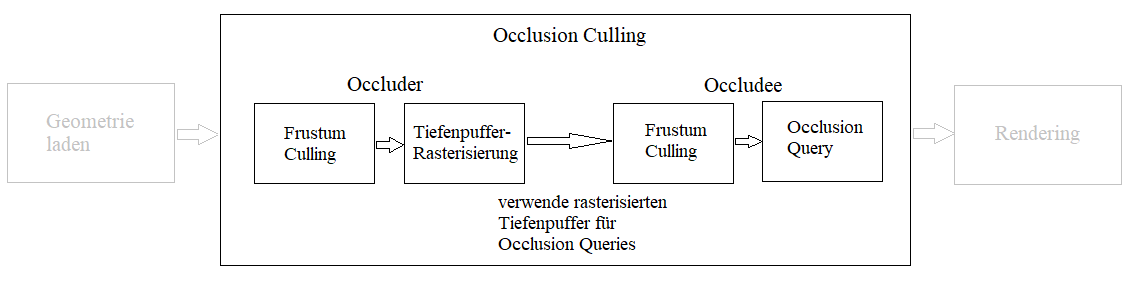
\includegraphics[width=\columnwidth]{images/SOCAblauf3.png}%
\caption{SOC-Ablauf: Nach Laden der Occludermenge wird im ersten Schritt durch Rasterisieren der Occluder der Tiefenpuffer generiert. Im zweiten Schritt werden die Occlusion Queries gestartet, die durch Rasterisierung und Tiefentests bestimmen, welche Objekte der Occludee-Menge sichtbar sind und welche nicht. Die Ergebnismenge wird an den Renderer weitergeleitet.}%
\label{fig:socablauf}%
\end{figure}


\subsection{Frustum Culling}
Frustum Culling l"asst nur Objekte passieren, die sich im Sichtbereich der Kamera befinden und kann somit je nach Kameraposition einen gro{\ss}en Teil der Objekte aus der Menge der zu rendernden Objekte herausnehmen.
Daf"ur wird die AABB des Objekts gegen jede der sechs Ebenen des Frustums getestet, ob sich die AABB \textit{vollst"andig} au{\ss}erhalb einer dieser Ebenen befindet.
Ist das der Fall, kann das Objekt als nicht sichtbar markiert werden und wird im weiteren Verlauf nicht weiter betrachtet. Dieser Zwischenschritt ist zwar optional, ist aber den Rechenaufwand wert, denn er bringt eine enorme Leistungssteigerung von teilweise "uber 200\%.\\
\textbf{(Optional! Vielleicht an anderer Stelle?)} Anmerkung zum Frustum Culling: W"ahrend die Performance des Frustum Cullings sehr konstant bleibt, sind bei anderen Occlusion Culling Algorithmen gr"o\ss{}ere Schwankungen erkennbar, da ein gro\ss{}er Occluder im Vordergrund potenziell alle Occludees hinter ihm "uberdecken kann und damit die Berechnung stark vereinfacht \cite{MSOC}.\\


\subsection{Tiefenpuffer Rasterisierung}
Alle Occluder, die nach dem Frustum Culling als sichtbar markiert sind, werden in diesem Schritt verwendet, um einen Tiefenpuffer zu generieren.
Dazu werden alle sichtbaren Objekte als eine Occludermenge \glqq gerendert\grqq{} (es wird lediglich ein Tiefenpuffer erzeugt ohne die Objekte tats"achlich zu zeichnen).
Das Rendering rasterisiert die Occluder, das hei{\ss}t, die Occluder werden auf den Bildschirm (screen space) transformiert und erzeugt anschlie{\ss}end den Tiefenpuffer, indem an den Stellen auf dem Bildschirm, an denen sich das Objekt befindet, die Tiefenwerte des Objekts gespeichert werden, siehe Abb.\ \ref{fig:db}.
\begin{figure}%
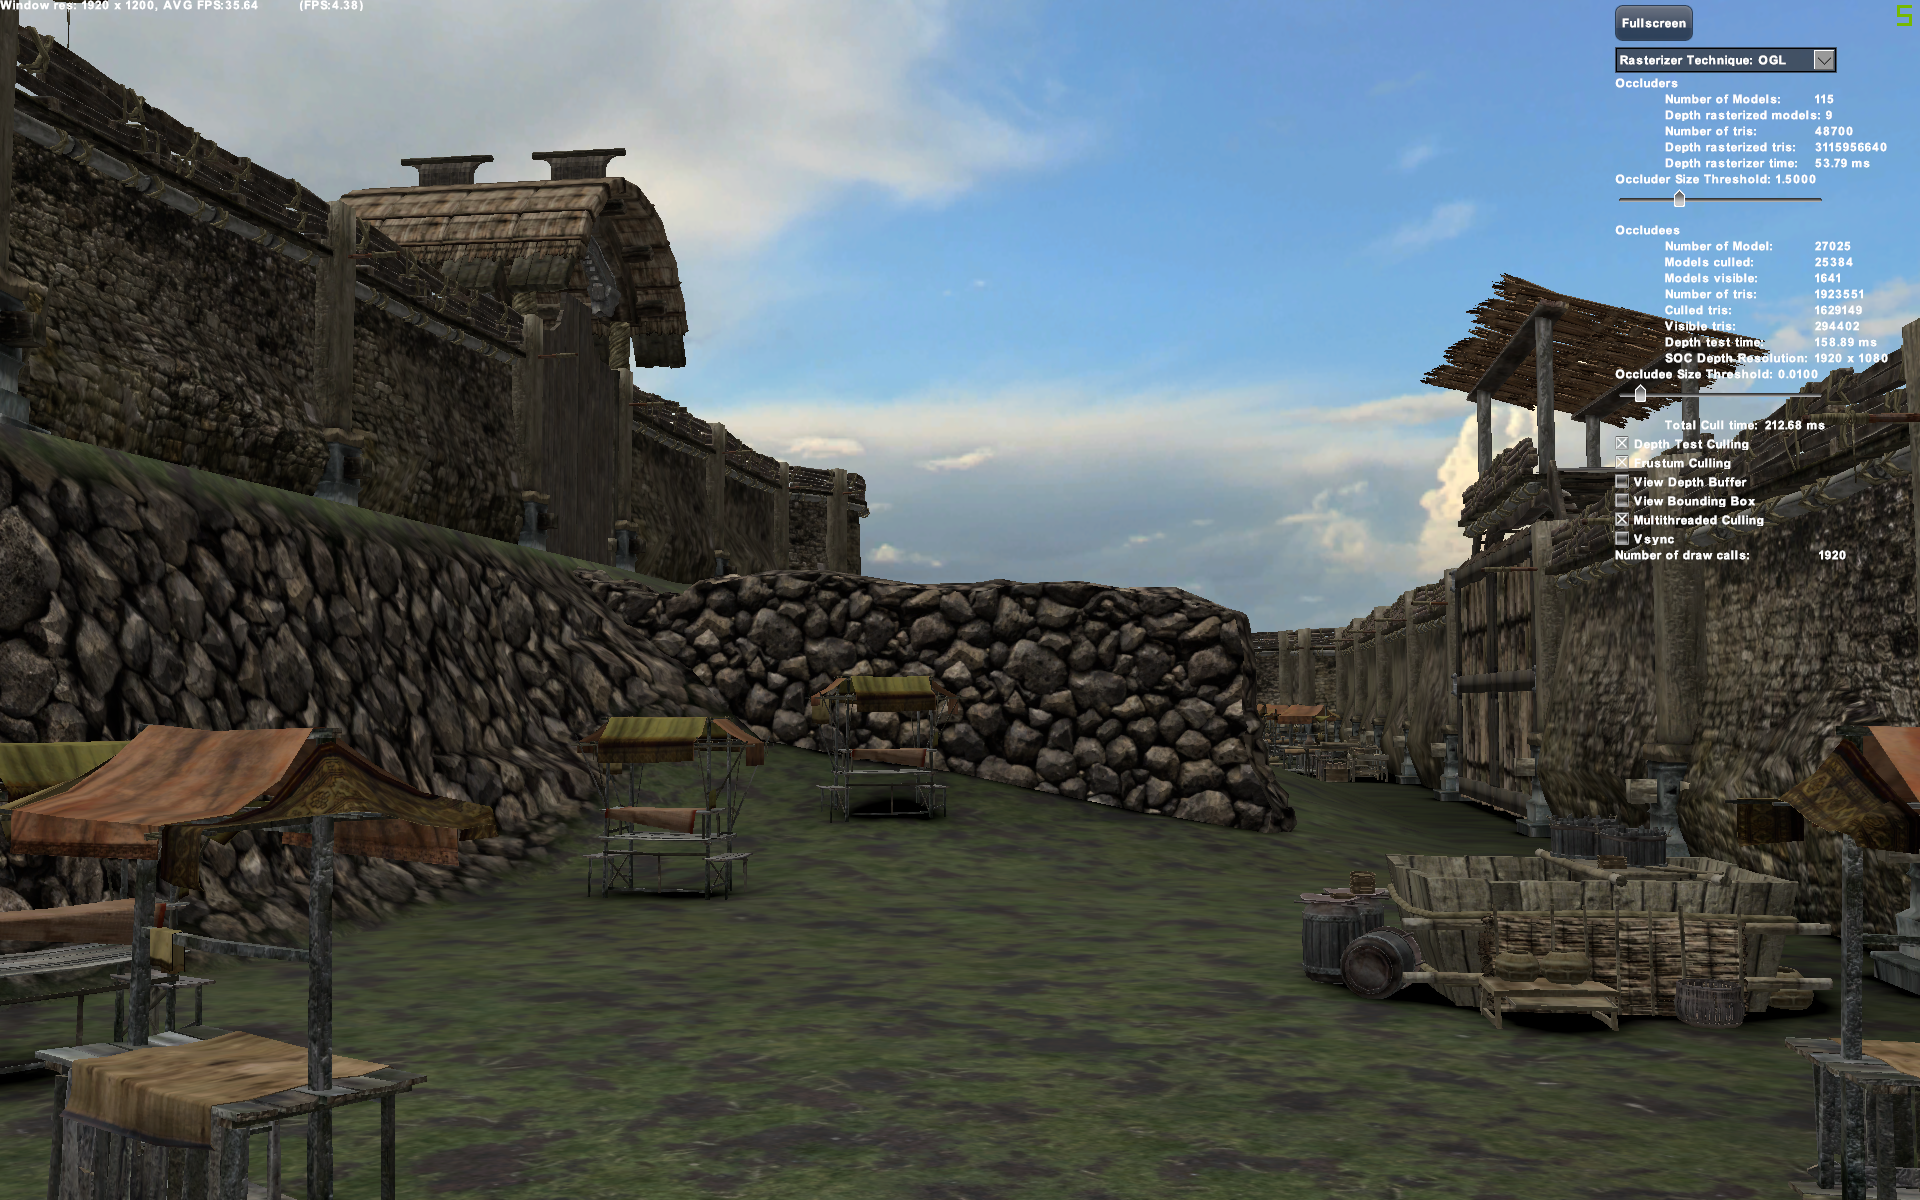
\includegraphics[width=0.5\columnwidth]{images/Base1.png}%
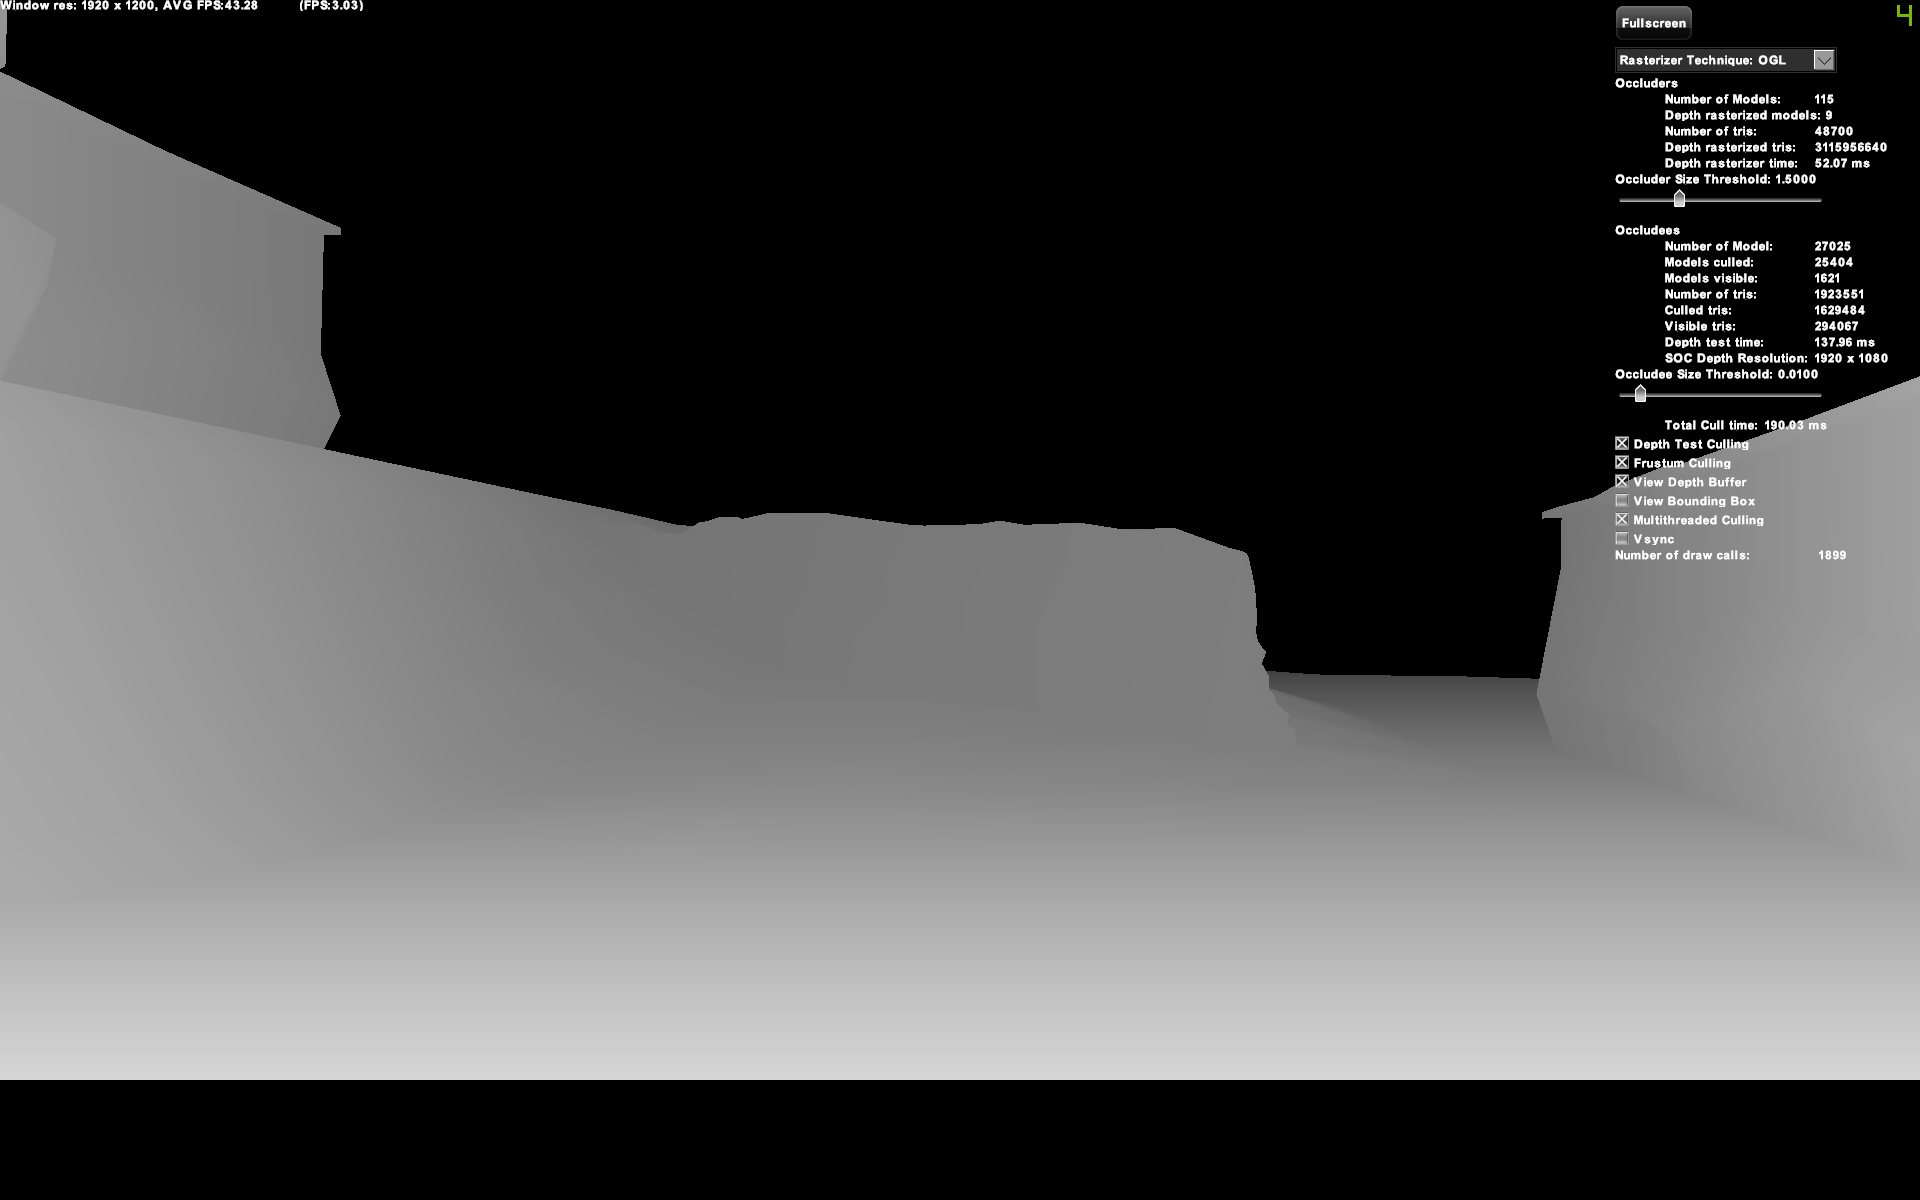
\includegraphics[width=0.5\columnwidth]{images/Base1DB.png}%
\caption{Links: Testbild der Szene. Rechts: Der dazugeh"orige Tiefenpuffer, der in jedem Frame einmal berechnet wird und sp"ater f"ur die Tiefentests der Occlusion Queries verwendet wird. Der schwarze Balken unterhalb des Tiefenpuffers entsteht durch die Differenz zwischen Fensteraufl"osung 1920x1200 und Tiefenpuffer-Aufl"osung 1920x1080.}%
\label{fig:db}%
\end{figure}


\subsection{Occlusion Queries}
An dieser Stelle sei erw"ahnt, dass die gesamte Occludeemenge zu Beginn des Programms einmal hochgeladen wurde (wohin?) und im Programm selber nur via Indexlisten zugegriffen wird, so dass zus"atzliche Ladezeiten vermieden werden.
Die Realisierung der Occlusion Queries gestaltet sich durch die von der OpenGL API zur Verf"ugung gestellten \textit{glQuery} sehr unkompliziert.
Zu Anfang werden f"ur alle Occludees, die innerhalb des Frustums sind, eine Occlusion Query gestartet.
Die Occludees werden wie die Occluder rasterisiert, allerdings wird in diesem Schritt der Tiefenpuffer nicht "uberschrieben, sondern es wird ausschlie{\ss}lich getestet, ob der Tiefenwert des Occludees kleiner als der des Tiefenpuffers ist.
Die Occlusion Query testet also, ob ein Teil des Occludees bei einem potenziellen Renderdurchlauf sichtbar w"are.
In diesem Fall liefert die Occlusion Query \glqq true\grqq{} zur"uck, andernfalls \glqq false\grqq{}.
Nachdem alle Occlusion Queries ihre Berechnungen beendet haben, werden zum Schluss alle Ergebnisse abgefragt und an das Framework f"ur den weiteren Renderingverlauf weitergeleitet.


%%%%%%%%%%%%%%%%%%%%%%
%%%%% ERGEBNISSE %%%%%
%%%%%%%%%%%%%%%%%%%%%%
\section{Ergebnisse}
Die dokumentierten Ergebnisse wurden mit dem SOC-Framework von Intel berechnet und verwenden die dortige Testszene einer Burg beziehungsweise eines Markplatzes, siehe Abb.\ \ref{fig:teaser}.
Die Burg umfasst 115 Occluder mit 48700 Dreiecken und 27025 Occludees mit $\approx$ 1923000 Dreiecken \cite{MSOC}. Sofern nicht anders angeben, wurden s"amtliche Ergebnisse mit einer Kamerafahrt, wie sie in Abb.\ \ref{fig:fahrt} angedeutet ist, "uber 100 Frames erstellt.
\begin{figure}%
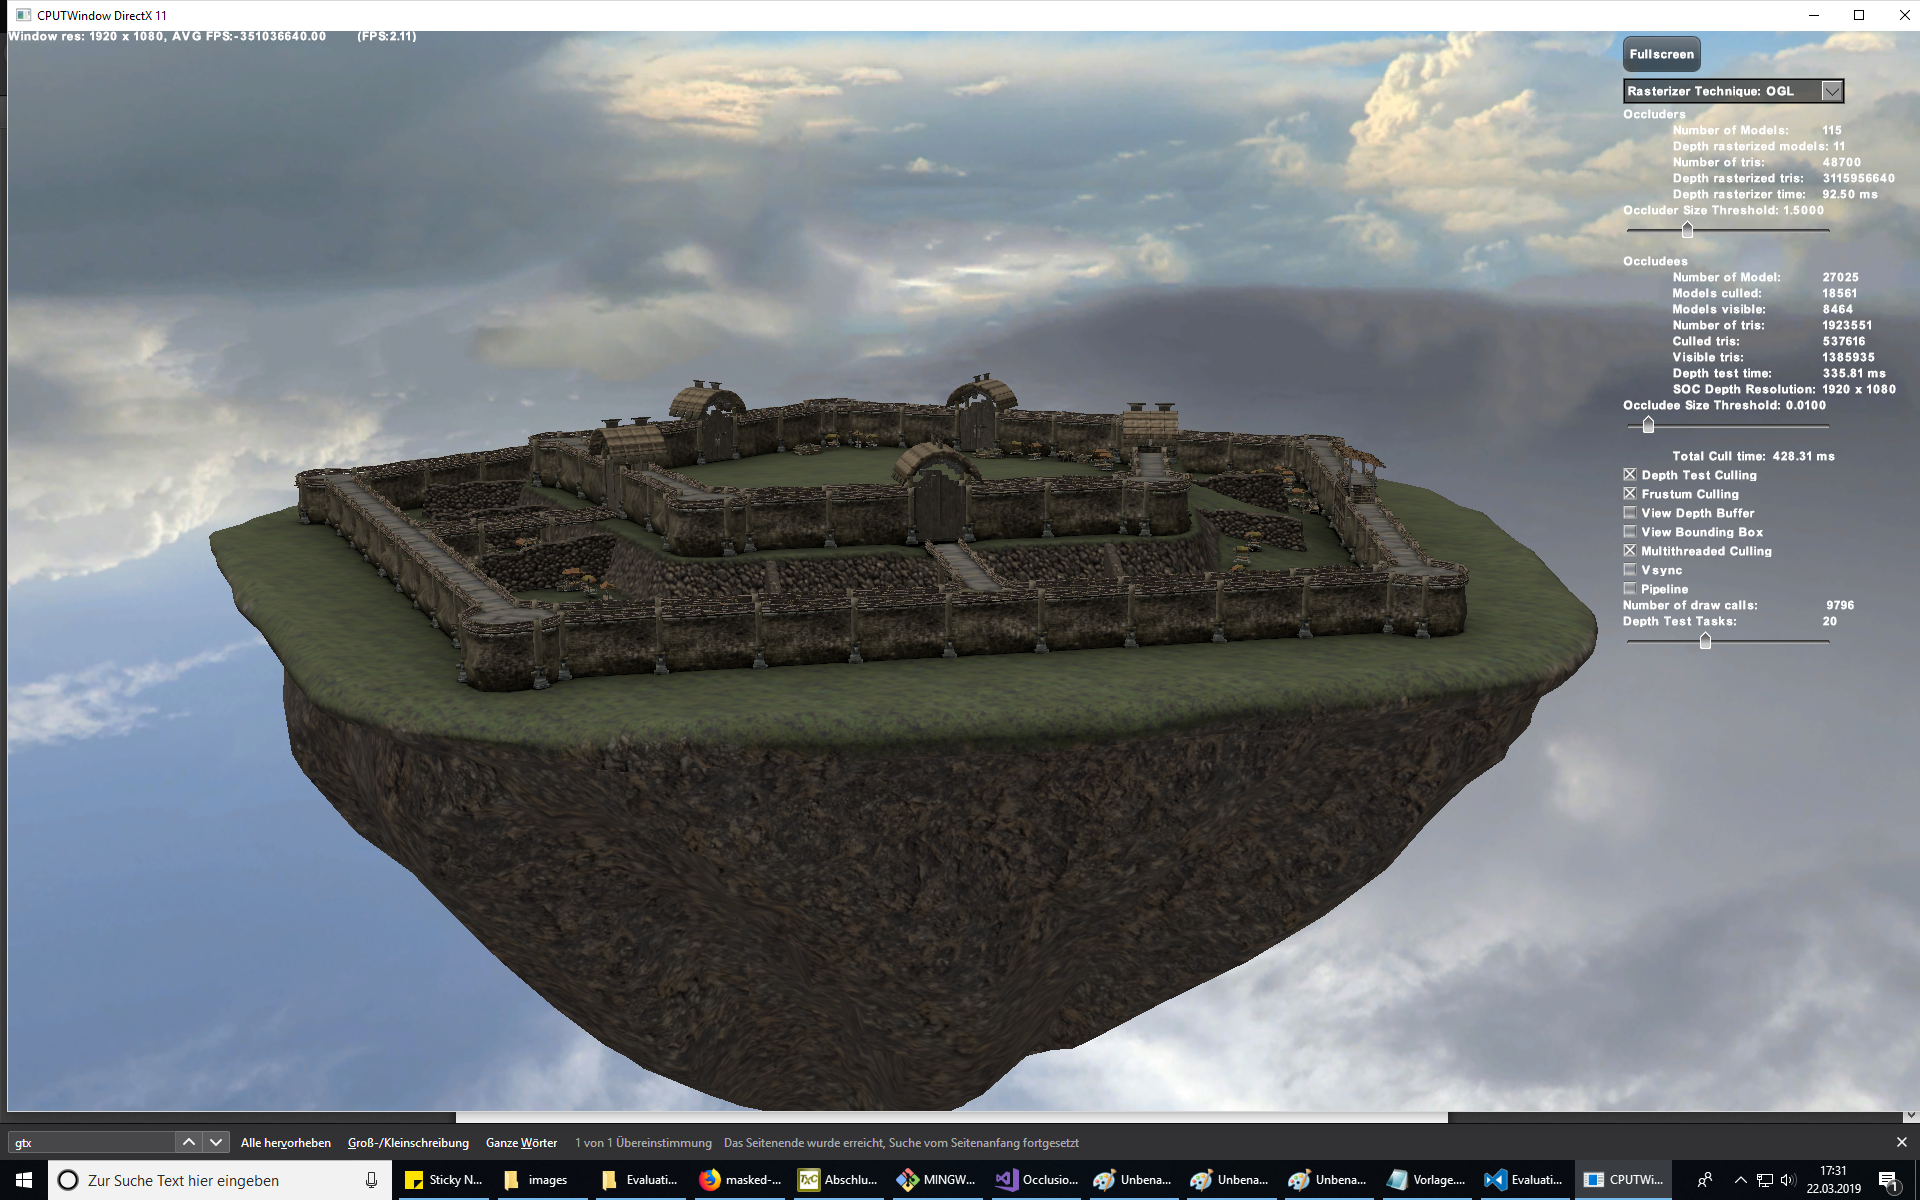
\includegraphics[width=0.33\columnwidth]{images/Tour1.png}%
\includegraphics[width=0.33\columnwidth]{images/Tour2.png}%
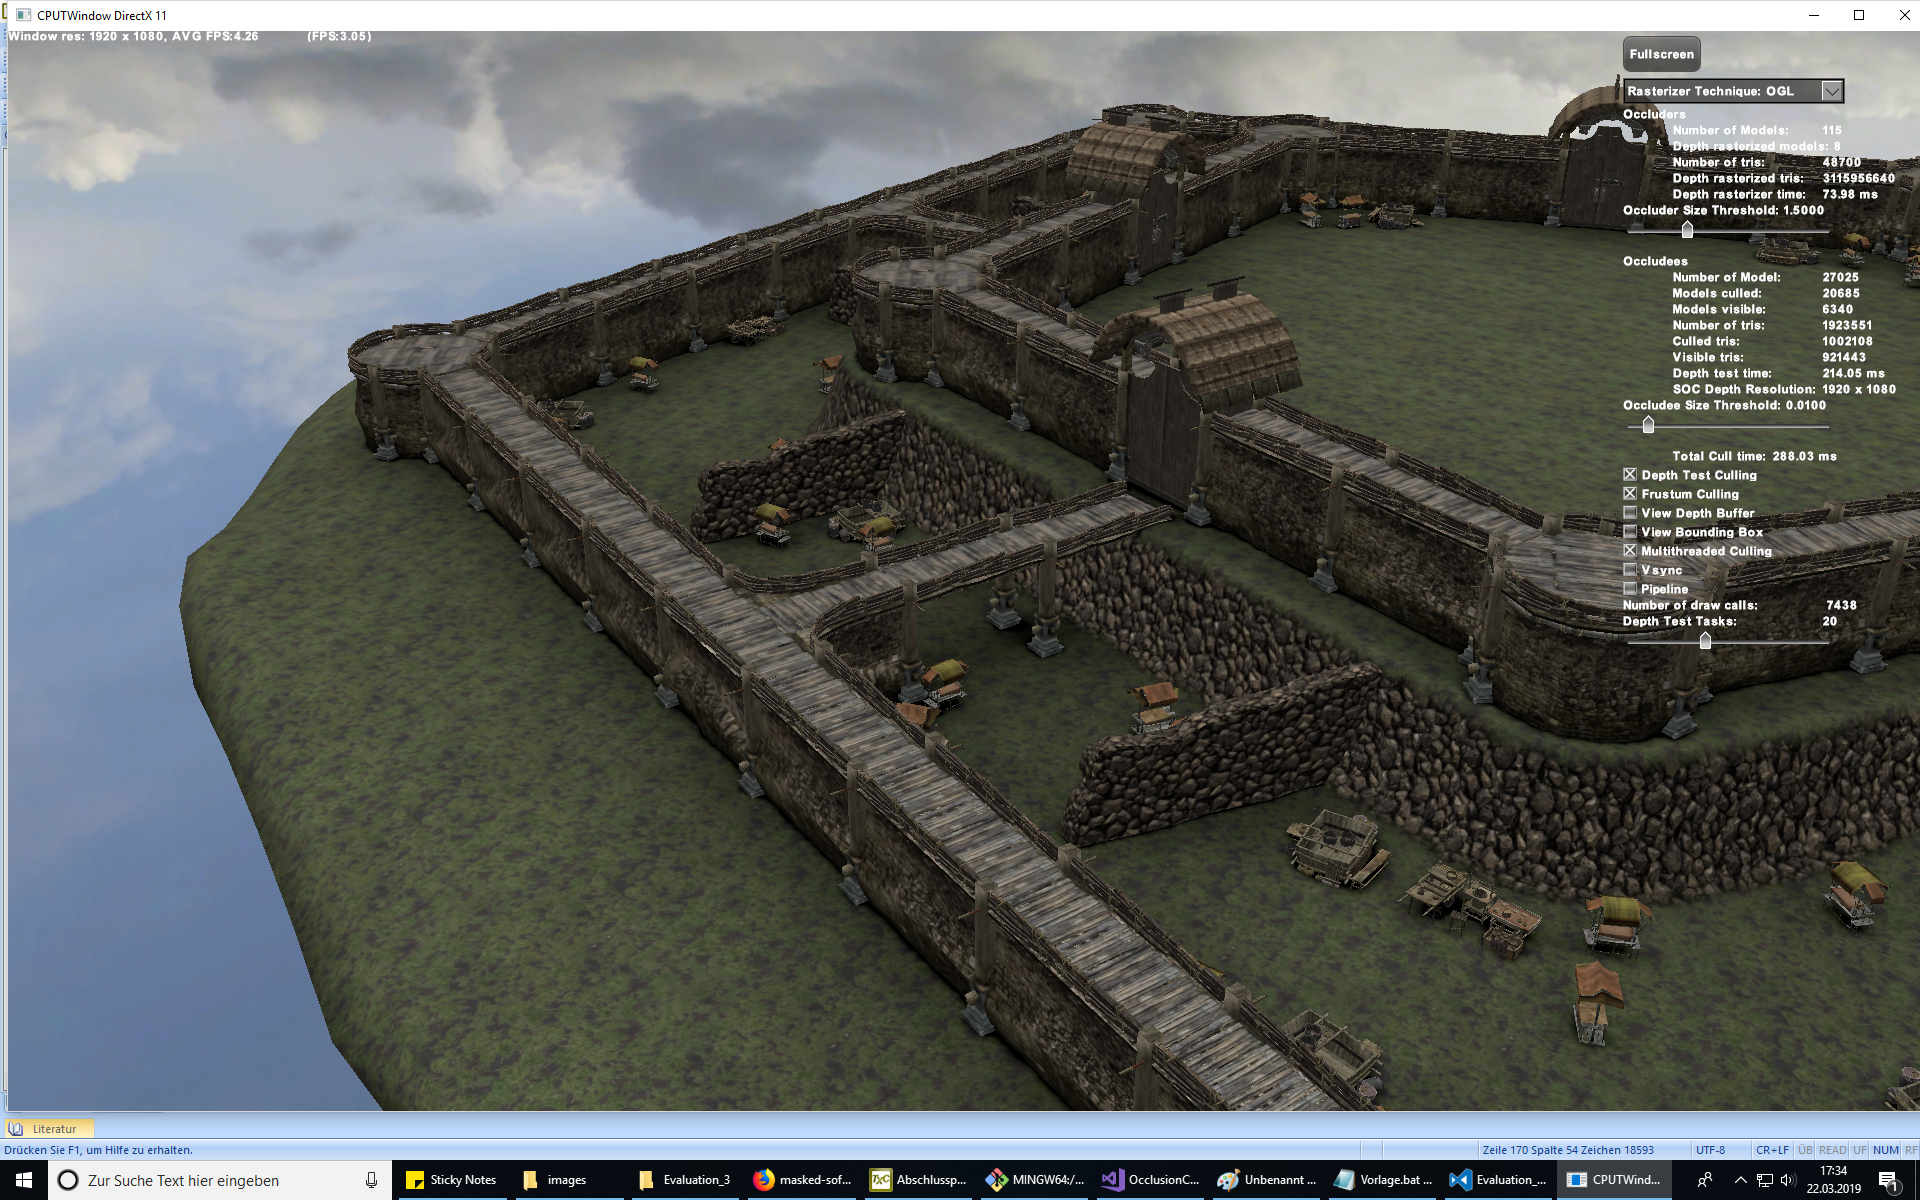
\includegraphics[width=0.33\columnwidth]{images/Tour3.png}%
\caption{Links: Startposition der Kamerafahrt. Mitte: n"ahert sich in einem Kreisbogen der Br"ucke an. Rechts: Die Kamera verl"asst die Szene in gleichem Bogen, wie sie sich angen"ahert hat.}%
\label{fig:fahrt}%
\end{figure}
Der Tiefenpuffer ist standardm"a"sig auf eine Aufl"osung von 1920x1080 Pixel gesetzt und au"serdem sind Multithreading, Frustum Culling und Occlusion Culling eingeschalten.
Die Kamera startet mit Blick auf die Burg aus einiger Entfernung und fliegt auf die Burg zu.
An der Burg angekommen dreht sich die Kamera in Richtung Boden und entfernt sich anschlie"send wieder von der Burg.
Die Anzahl der Objekte im Sichtfeld ist am Anfang sehr hoch, sinkt in der Mitte der Kamerafahrt ab und steigt am Ende wieder auf den Startwert.
Als Hardware wurde ein Rechner mit einem Intel Core i7-4770, einer NVIDIA Geforce GTX 960 und 16 GB RAM verwendet.\\

%%%%%%%%%%%%%%%%%%%%%%%%%%%%%%%%%%%%%%%%%%%%%%%%%%%%%%%%%%%%%%
%%%%%%%%%%%%%%%%%%%% TRIES CULLED BEGIN %%%%%%%%%%%%%%%%%%%%%%
%%%%%%%%%%%%%%%%%%%%%%%%%%%%%%%%%%%%%%%%%%%%%%%%%%%%%%%%%%%%%%
Zuerst wurde die OGL-Methode auf den qualitativen Aspekt untersucht, das hei"st, ist das Ergebnis korrekt und wie \glqq gut\grqq{} ist das Ergebnis im Hinblick auf die Anzahl der weggeworfenen Dreiecke.
Abb.\ \ref{fig:resolution_culled} zeigt die erzielten Ergebnisse.
Im linken Bild ist ein Vergleich aller im SOC-Framework implementierten Occlusion Culling Techniken zu finden.
Es ist gut zu sehen, dass die OGL-Methode qualitativ keinerlei Abstriche bei dieser Eigenschaften gegen"uber den anderen Techniken machen muss.
Lediglich die etwas schlechteren Werte der MOC-Methode stehen hervor, aber das ist nicht verwunderlich, da dies bereits in \cite{MSOC} erl"autert wurde.
In einem weiteren Test, der nur die OGL-Methode betrifft, wurde untersucht, inwiefern eine geringere Aufl"osung des Tiefenpuffers Auswirkungen auf die Anzahl der weggeworfenen Dreiecke hat und somit indirekt ebenfalls Auswirkungen auf die Anzahl der Objekte, die weggeworfen werden und schlie"slich auf die Anzahl der Draw Calls, die einen wichtigen Teil der gesamten Performanz ausmachen.
Die Ergebnisse sind gr"osteils genau so zu erwarten.
Je geringer die Aufl"osung des Tiefenpuffers wird, desto gr"ober und ungenauer wird das Ergebnis, sprich mit fallender Aufl"osung steigt die Anzahl der Dreiecke, die weggeworfen werden.
Interessant ist das Ergebnis f"ur die Aufl"osung 1920x1080.
Zu Anfang ist der Verlauf "ahnlich zu allen anderen, aber etwa ab Frame 60 verringert sich die Anzahl an weggeworfenen Dreiecken ungef"ahr linear und nicht wie allen anderen ungef"ahr quadratisch.
\textbf{ERKL"ARUNG DAF"UR}.
Ebenfalls wie erwartet ist das Ergebnis f"ur die Anzahl an Objekten, die weggeworfen werden und die Draw Calls (siehe Abb.\ \ref{fig:resolution_culled} Tabelle).
Geht die Anzahl der weggeworfenen Objekte hoch, geht entsprechend die Anzahl der Draw Calls runter (und dar"uber hinaus verbessert sich entsprechend die Performanz, sp"ater mehr).
Lediglich die Anzahl an Draw Calls f"ur 1920x1080 entrinnt dem Muster, da es erwartungsgem"a"s weniger Draw Calls geben m"usste f"ur die Anzahl an weggeworfenen Dreiecken.\\

\begin{figure*}
	\begin{minipage}{\textwidth}
		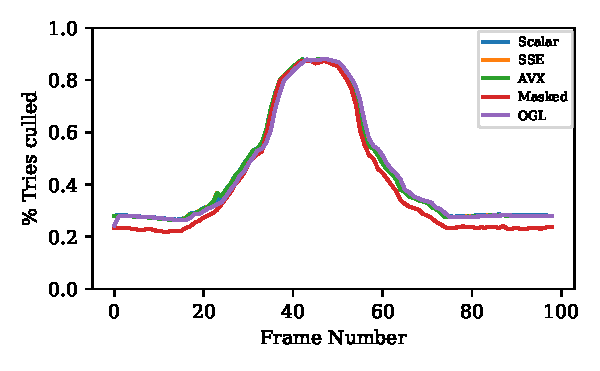
\includegraphics[width=0.5\textwidth]{images/Evaluation_1_Results_Percentage culled.pdf}
		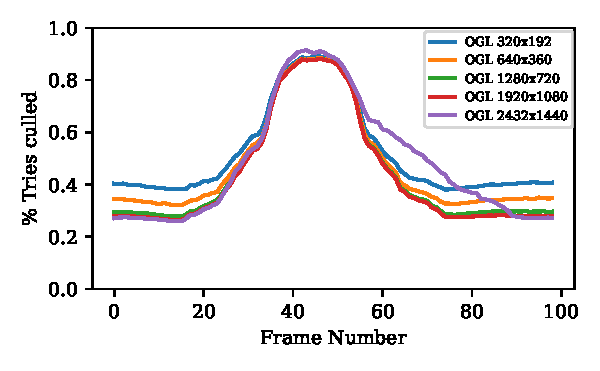
\includegraphics[width=0.5\textwidth]{images/Evaluation_4_Results_Percentage culled.pdf}
	\end{minipage}
	\begin{minipage}{\textwidth}
		\centering
		\scalebox{1.2}{
			\begin{tabular}{| l | r | r | r | r | r |}
				\hline
				& 320x192   & 640x360   & 1280x720  & 1920x1080 & 2432x1440 \\ \hline
				Tries culled (\%)    & 51.75     & 47.59     & 44.65     & 48.18     & 43.77     \\ \hline
				Draw Calls           & 3551      & 5696      & 7644      & 7896      & 8423      \\ \hline
				Models Culled        & 23819.61  & 21970.67  & 20320.78  & 20135.84  & 19660.16  \\ \hline
				Models Visible       & 3205.39   & 5054.33   & 6704.22   & 6889.16   & 7364.84   \\
				\hline
		\end{tabular}}
	\end{minipage}
	\caption{Im linken Diagramm ist die Prozentangabe der weggeworfenen Dreiecke mit den f"unf verschiedenen Methoden des SOC-Frameworks, bei einer Aufl"osung des Tiefenpuffers von 1920x1080, zu sehen. Im rechten Diagramm wird die Anzahl der weggeworfenen Dreiecke bei unserer OGL-Methode mit f"unf verschiedenen Aufl"osungen des Tiefenpuffers verglichen. Interessant zu beobachten ist der Verlauf f"ur die Aufl"osung 1920x1080, da er im abfallenden Bereich ungef"ahr linear und nicht ann"ahernd quadratisch verl"auft. Tabelle: Die Anzahl der Draw Calls ist bei 1920x1080 ebenfalls etwas au"serhalbs des Musters, vergleiche zum Beispiel mit 640x360.}
	\label{fig:resolution_culled}
\end{figure*}
%%%%%%%%%%%%%%%%%%%%%%%%%%%%%%%%%%%%%%%%%%%%%%%%%%%%%%%%%%%%%%
%%%%%%%%%%%%%%%%%%%% TRIES CULLED END %%%%%%%%%%%%%%%%%%%%%%%%
%%%%%%%%%%%%%%%%%%%%%%%%%%%%%%%%%%%%%%%%%%%%%%%%%%%%%%%%%%%%%%

%%%%%%%%%%%%%%%%%%%%%%%%%%%%%%%%%%%%%%%%%%%%%%%%%%%%%%%%%%%%%%
%%%%%%%%%%%%%%%%%%%% MT - FC - DT BEGIN %%%%%%%%%%%%%%%%%%%%%%
%%%%%%%%%%%%%%%%%%%%%%%%%%%%%%%%%%%%%%%%%%%%%%%%%%%%%%%%%%%%%%
Als n"achstes wurden die Auswirkungen verschiedener Culling Kombinationen auf die Anzahl der weggeworfenen Dreiecke und vor allem auf die Draw Calls untersucht, siehe Abb.\ \ref{fig:OGL_MOC_frustum_culling}.
L"auft die OGL-Methode ohne Frustum Culling und ohne das Ausf"uhren der Occlusion Queries, ist die Anzahl an Draw Calls entsprechend hoch, da die Anzahl an sichtbaren Objekten durch die fehlenden Culling-Mechaniken sehr hoch ist.
Interessant ist der H"ohepunkt in der Mitte der Kamerafahrt.
Wohingegen bei den anderen Kombinationen an dieser Stelle der niedrigste Wert erreicht wird, ist er dort ohne Frustum Culling und ohne Occlusion Queries am h"ochsten.
Besser wird das Ergebnis, wenn zus"atzlich zum Multithreading das Frustum Culling aktiviert wird.
Je n"aher die Kamera sich der Burg n"ahert, desto h"oher ist die Anzahl weggeworfener Objekten und die Menge an Draw Calls f"allt entsprechend auf ihren Tiefstwert und steigt anschlie"send wieder mit Distanz der Kamera zur Burg.
Sind sowohl Frustum Culling als auch Occlusion Queries aktiviert, ist der Verlauf der im Prinzip der Gleiche, mit dem Unterschied, dass die Menge an Draw Calls zu Anfang und zum Schluss deutlich niedriger ist.
Sind es ohne Occlusion Queries zu Anfang rund 17000 Objekte, die gerendert werden m"ussen, so sind es mit Occlusion Queries in etwa 6000-7000 weniger, womit Occlusion Queries einen enormen Renderingaufwand einsparen.\\
\textbf{Vergleich mit MOC fehlt noch}.\\
%%%%%
Da die verschiedenen Methoden nur f"ur den Tiefentest benutzt werden, sind die Werte ohne den Tiefentest unabh"angig von der Methode.
Erst beim aktivierten Tiefentest lassen sich unterschiede erkennen, wie bereits in \ref{fig:resolution_culled} festgestellt wirft die MOC.Methode etwas weniger Dreiecke weg.
Aus mehr sichtbaren Dreiecken resultieren dann auch mehr Drawcalls.
%%%%%

\begin{figure*}
	\begin{minipage}{0.4\textwidth}
		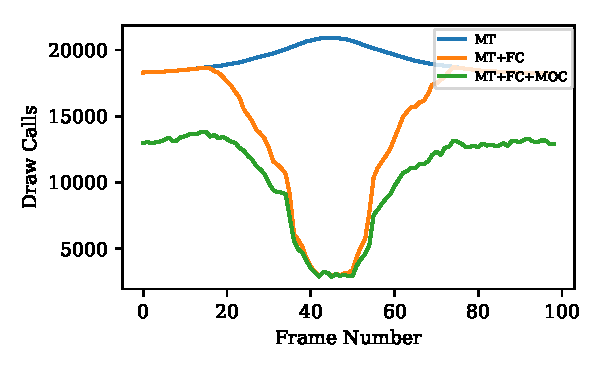
\includegraphics[width=\textwidth]{images/Evaluation_7_Results_MOC_Draw Calls.pdf}
	\end{minipage}
	\begin{minipage}{0.4\textwidth}
		\centering
		\scalebox{1.2}{
			\begin{tabular}{| l | r | r | r | r | r |}
				\hline
				& MT        & MT+Frustum& MT+Frustum\\
				&           &           & + Depth Test\\ \hline
				Tries culled (\%)    & 11.13     & 11.13     & 40.41     \\ \hline
				Draw Calls           & 19219     & 14318     & 10528     \\ \hline
				Models Culled        & 10180.34  & 14532.39  & 17903.78  \\ \hline
				Models Visible       & 16844.66  & 12492.61  & 9121.22   \\
				\hline
		\end{tabular}}
	\end{minipage}
	
	\begin{minipage}{0.4\textwidth}
		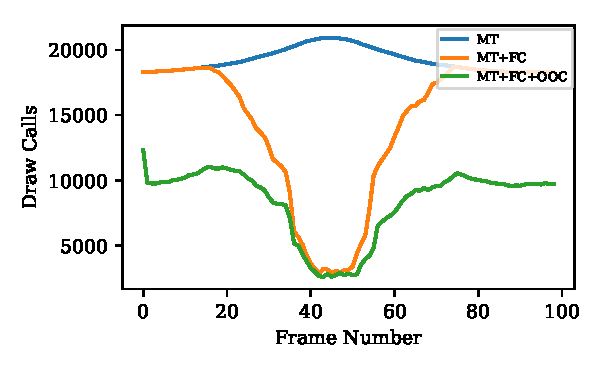
\includegraphics[width=1\textwidth]{images/Evaluation_7_Results_OGL_Draw Calls.pdf}
	\end{minipage}
	\begin{minipage}{0.4\textwidth}
		\centering
		\scalebox{1.2}{
			\begin{tabular}{| l | r | r | r | r | r |}
				\hline
				& MT        & MT+Frustum& MT+Frustum\\
				&           &           & + Depth Test\\ \hline
				Tries culled (\%)    & 11.13     & 11.13     & 43.77     \\ \hline
				Draw Calls           & 19219     & 14318     & 8423      \\ \hline
				Models Culled        & 10180.34  & 14532.39  & 19660.16  \\ \hline
				Models Visible       & 16844.66  & 12492.61  & 7364.84   \\
				\hline
		\end{tabular}}
	\end{minipage}
	\caption{Vergleich Anzahl Draw Calls von Multi-Threading (MT), MT + Frustum Culling (FC) und MT + FC + Tiefentest Culling (TTC). Anzahl Draw Calls geht mit Verlauf der Kamerafahrt mit FC und TTC deutlich runter. Ist TTC aktiviert, werden sind die Maximalwerte am Anfang und Schluss deutlich niedriger. \textbf{Vergleich mit MOC fehlt noch}}
	\label{fig:OGL_MOC_frustum_culling}
\end{figure*}
%%%%%%%%%%%%%%%%%%%%%%%%%%%%%%%%%%%%%%%%%%%%%%%%%%%%%%%%%%%%%%
%%%%%%%%%%%%%%%%%%%% MT - FC - DT END %%%%%%%%%%%%%%%%%%%%%%%%
%%%%%%%%%%%%%%%%%%%%%%%%%%%%%%%%%%%%%%%%%%%%%%%%%%%%%%%%%%%%%%

%%%%%%%%%%%%%%%%%%%%%%%%%%%%%%%%%%%%%%%%%%%%%%%%%%%%%%%%%%%%%%
%%%%%%%%%%%%%%%%%%%%%%%% FPS BEGIN %%%%%%%%%%%%%%%%%%%%%%%%%%%
%%%%%%%%%%%%%%%%%%%%%%%%%%%%%%%%%%%%%%%%%%%%%%%%%%%%%%%%%%%%%%
Als letztes wurde der wohl wichtigste Aspekt untersucht, die Performanz im Vergleich mit anderen SOC-Methoden im Intel-Framework.
Trotz der guten Werte, die die OGL-Methode in den Tests  davor erzielt, schneidet sie im Leistungsstest sehr schlecht ab.
Getestet wurden alle Methoden mit aktiviertem Multithreading, Frustum Culling und Tiefentest Culling. Abb.\ \ref{fig:resolution_fps} zeigt den Leistungsvergleich mit den anderen SOC-Methoden.
Es ist gut zu sehen, dass die FPS bei allen Methoden im Bereich circa zwischen Frame 35 und 55 stark anstiegen sind.
In diesem Bereich werden mehr Objekte weggeworfen und die Anzahl an Draw Calls verringert sich, deswegen sind dort mehr FPS m"oglich.
Ebenfalls deutlich zu erkennen ist, das die OGL-Methode viel weniger FPS w"ahrend der gesamten Fahrt hat als alle anderen.
Wohingegen sich der Rest zu Beginn und gegen Ende um die $120\pm20$ FPS befindet, ist die OGL-Methode bei circa 3 FPS anzutreffen.
Ein "ahnliches Bild ergibt die Analyse der Spitzenwerte.
Der Maximalwert bei OGL ist bei knapp 16 FPS, w"ahrend sich die anderen Methoden bei circa 280-380 FPS aufhalten (lediglich die Scalar-Methode befindet sich nicht in diesem Spitzenbereich).
Diese schlechten FPS-Werte sind nicht verwunderlich, wenn die Zeiten f"ur das Rasterisieren und die Tiefentests in der Tabelle aus Abb.\ \ref{fig:resolution_fps} betrachtet werden.
So hat die OGL-Methode bei einer Aufl"osung von 1920x1080 durchschnittliche Werte von 265ms f"ur Tiefentests und 7ms Rasterisierungszeit.
Zum Vergleich, die Werte beim MOC liegen bei ungef"ahr 0.1ms f"ur die Rasterisierung und 0.39ms f"ur Tiefentests.\\

Es wurde auch ein Test durchgef"uhrt, der das Leistungsverhalten unterschiedlicher Tiefenpuffer-Aufl"osungen untersucht.
Im rechten Bild von Abb.\ \ref{fig:resolution_fps} sind die verschiedenen Verl"aufe zu sehen.
Je geringer die Aufl"osung wird, desto h"oher werden die Bildraten, die teilweise fast viermal so hoch sind, wenn zum Beispiel die Mitte der Kamerafahrt betrachtet wird.
So kommt die Full-HD Aufl"osung 1920x1080, im Gegensatz zu den knapp "uber 21 FPS bei der sehr niedrigen Aufl"osung von 320x192, auf gerade einmal knapp "uber 4 FPS. Der Preis daf"ur ist allerdings ein durchaus schlechteres Ergebnis.
Bei geringer Aufl"osung (z. B. 640x360) ist deutlich zu erkennen, dass einige Objekte fehlen, die bei h"oheren Aufl"osungen sichtbar sind.
Eine Ausnahme findet sich bei der 2432x1440 Aufl"osung.
Sie schneidet, entgegen dem Trend der niedriger werdenden FPS bei steigender Aufl"osung, besser ab, als die Full-HD Aufl"osung.\\

\begin{figure*}
	\begin{minipage}{\textwidth}
		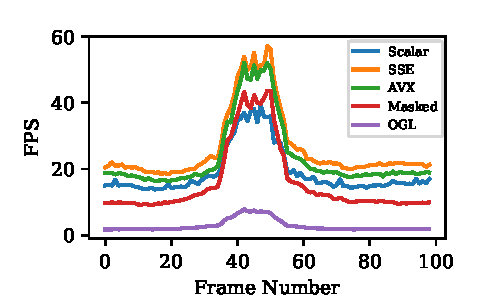
\includegraphics[width=0.5\textwidth]{images/Evaluation_1_Results_FPS.pdf}
		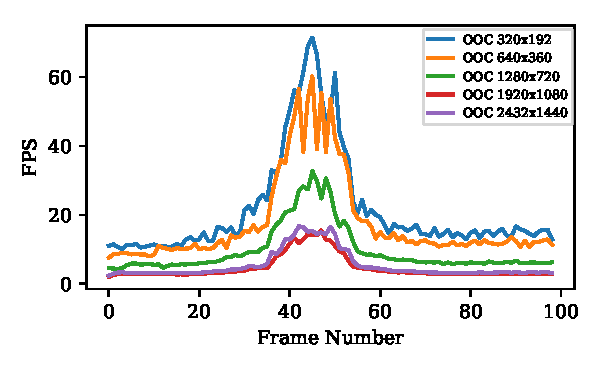
\includegraphics[width=0.5\textwidth]{images/Evaluation_4_Results_FPS.pdf}
	\end{minipage}
	\begin{minipage}{\textwidth}
		\centering
		\scalebox{1.2}{
			\begin{tabular}{| l | r | r | r | r | r |}
				\hline
				& 320x192   & 640x360   & 1280x720  & 1920x1080 & 2432x1440 \\ \hline
				FPS                  & 21.48     & 17.53     & 9.55      & 4.58      & 5.31      \\ \hline
				DepthTest time (ms)  & 50.4      & 63.22     & 122.21    & 265.67    & 228.85    \\ \hline
				Rasterize time (ms)  & 6.64      & 6.85      & 6.87      & 7.07      & 8.02      \\
				\hline
		\end{tabular}}
	\end{minipage}
	\caption{Links: FPS-Vergleich aller SOC-Methoden im Intel-Framework bei Full-HD Aufl"osung, aktiviertem MT, FC und TTC. OGL schneidet mit teilweise circa nur einem F"unftel der FPS von MOC oder SSE deutlich am schlechtesten ab. Rechts: Kamerafahrt mit unterschiedlichen Tiefenpuffergr"o"sen. Mit niedriger werdenden Aufl"osungen sinken die Tiefentestzeiten ab (siehe Tabelle) und die FPS steigen erwartungsgem"a"s an, mit einer Ausnahme bei der 4k-Aufl"osung, die trotz ihrer 4-fachen Full-HD Puffergr"o"se, besser abschneidet als die Full-HD Aufl"osung.}
	\label{fig:resolution_fps}
\end{figure*}
%%%%%%%%%%%%%%%%%%%%%%%%%%%%%%%%%%%%%%%%%%%%%%%%%%%%%%%%%%%%%%
%%%%%%%%%%%%%%%%%%%%%%%% FPS END %%%%%%%%%%%%%%%%%%%%%%%%%%%%%
%%%%%%%%%%%%%%%%%%%%%%%%%%%%%%%%%%%%%%%%%%%%%%%%%%%%%%%%%%%%%%

\paragraph{Anmerkung} An dieser Stelle ist es auch im R"uckblick auf Abb.\ \ref{fig:OGL_MOC_frustum_culling} interessant, anzumerken, dass die Performanz am besten ist, wenn sowohl Frustum Culling als auch Tiefentest Culling deaktiviert sind. In der Standard-Kameraeinstellung werden durchschnittlich 91 FPS erreicht. Wird nur Frustum Culling aktiviert, werden im Schnitt 84 FPS erreicht.
Je nach Kameraposition erreicht Frustum Culling jedoch stellenweise auch höhere Frameraten.
Wird zus"atzlich noch das Tiefentest Culling aktiviert, f"allt der Wert auf 5 FPS.\\

\paragraph{Probleme} Die gr"o"sten Performanzprobleme werden durch die Occlusion Queries verursacht.
Das Programm wurde mit einem Performance Profiler analysiert, um herauszufinden, an welchen Stellen das Programm viel Zeit verbraucht und die meiste Zeit h"alt sich das Programm bei den Occlusion Queries auf.
Das ist teilweise auch so zu erwarten, da die Occlusion Queries ein essentieller Teil des Programms sind. Dennoch wird dort zu viel Zeit verbracht, vor allem der Tatsache geschuldet, dass der Prozessor nicht mehr als 50\% ausgelastet ist und damit nicht seine gesamte Kapazit"at in Anspruch nimmt.
Ein Grund f"ur den gro"sen Zeitverlust wurde bei langen Wartezeiten gesehen, die entstanden sind, nachdem alle OQ gestartet wurden und das Programm auf die Ergebnisse warten musste.
Deswegen wurde die Implementierung dahingehend ge"andert, dass ein zweites Set an Occlusion Queries generiert wurde, das die Ergebnisse der OQs des vorherigen Frames enth"alt.
Durch das zweite Set kann die Warteroutine weggelassen werden, unter der Annahme, dass im aktuellen Frame alle Ergebnisse des vorherigen Frames vorliegen.
Dadurch konnte das Problem mit langen Wartezeiten zwar gel"ost werden, allerdings wurden dadurch keine signifikanten Performanzverbesserungen erzielt.
Wieso brauchen OQ so lange?


%Notizen zu den Ergebnissen:
%%%%%%%%%%%%%%%%%%%%%%%%%%%%%%%%%%%%%%%%%%%%%%
%Evaluation 1: alle 5, Kamerafahrt 1\\
%Evaluation 2: alle 5, Kamerafahrt 2\\
%Evaluation 3: alle 5, DB\_Very\_Large vs DB\_Small\\
%Evaluation 4: OGL, alle 5 Aufl"osungen\\
%Evaluation 5: OGL, mit und ohne Frustum culling\\
%Evaluation 6: alle 5 + OGL ohne Mesa\\
%Evaluation 7: OGL + SSE, MT / MT + Frustum Culling / MT + Frustum Culling + Depth Test Culling\\
%Evaluation 8: OGL + SSE, Depth Test Tasks 5 / 20 / 100
%Evaluation 9: OGL, OccluderPerQuery 0 / 1 / 2 / 3 / 5 / 10 / 15
%
%1)
%- Auflösungen DB
%- Diagramm: Percentage culled Evaluation 1 + 4 nebeneinander
%- Tabelle: \% Culled, Drawcalls, Models Culled, Models Visible
%
%2)
%- MT/MT+Frustum/MT+Frustum/DP
%- Diagramm: Drawcalls OGL + MOC
%- Tabelle: Models Visible, Models Culled, Drawcalls, \% Culled tries
%
%3)
%- Auflösungen DB
%- Diagramm: Frames alle
%- Diagramm: Frames OGL Auflösungen
%- Tabelle:  Frames, DT time, Rasterizer time
%
%Optional:
%5)
%- Future Work
%- Mehrere Occluder gleichzeitig rendern 
%6) OGL vs ohne Mesa
%7) Depth Test Task 1-100
%8) Occluder Threshold
%9) Occludee Threshold
%%%%%%%%%%%%%%%%%%%%%%%%%%%%%%%%%%%%%%%%%%

\section{Fazit}
In dieser Arbeit wurde gezeigt, dass es mit Hilfe von Mesa 3D m"oglich ist, eine Occlusion Culling Methode zu entwickeln, die parallel zum GPU-Rendering auf dem Prozessor l"auft.
Die Auswertung hat gezeigt, dass die neu entwickelte OGL-Methode qualitativ, im Sinne von weggeworfenen Dreiecken beziehungsweise Objekten, mit den bereits vorhandenen SOC-Methoden konkurrieren kann.
Unter dem Aspekt der Performanz kann die OGL-Methode allerdings nicht mit den anderen mithalten.  \\

\paragraph{Future Work} Zuk"nftige Arbeiten k"onnen sich damit besch"aftigen, Occludees zu Paketen zu schn"uren und lediglich eine Occlusion Query mit dem Paket zu starten, anstatt wie bisher f"ur jedes Objekt eine separate Query durchzuf"uhren.
Ziel ist es, weniger Occlusion Queries zu generieren, ohne dabei zu viel an Qualit"at einb"u"sen zu m"ussen und dadurch an Performanz zu gewinnen.
Die Auswahl der Occludees, die zu einem Paket zusammengeschn"urt werden ist dabei von gro"ser Wichtigkeit und entscheidend f"r das Ergebnis, sowohl im Hinblick auf die Performanz, als auch auf die Korrektheit des Ergebnisses (werden alle Occludees angezeigt, die sichtbar sind oder fehlen Objekte in der Szene).
Die Auswahl der Objekte sollte dabei so vonstattengehen, dass nur Occludees zu einem Paket zusammengefasst werden, die sich in einer bestimmten (kleinen) Region befinden, so dass Pakete vermieden werden, bei denen die Objekte "uber gro"se Teile der Szene verteilt sind.
Eine erste Version dieser Technik wurde bereits implementiert und ein erster Test hat ergeben, dass eine Performanzverbesserung durchaus m"oglich ist, allerdings leidet das Ergebnis erheblich an Qualit"at, da es aktuell oft vorkommt, dass Occludee-Pakete so geschn"urt werden, dass Objekte f"alschlicherweise aus der Liste der zu rendernden Objekte geworfen werden.
Mit einem optimierten Auswahlverfahren k"onnen auf die Weise wahrscheinlich deutliche Verbesserungen erzielt werden sowohl im Performanzbereich als auch bei der Qualit"at des Ergebnisses. 

\bibliographystyle{abbrv} 
%% use following if all content of bibtex file should be shown
% \nocite{*}
\bibliography{literatur}
\end{document}
